\documentclass[a4j]{jsarticle}
%
% 古いパッケージを自動チェック
\RequirePackage[l2tabu, orthodox]{nag}
\usepackage[all, warning]{onlyamsmath}
% 古いパッケージを自動チェック

%\usepackage{subcaption} %図の中に複数の図を入れる
\usepackage[top=30mm,bottom=30mm,left=25mm,right=25mm]{geometry}% 幅160mmの余り
\usepackage{url} %URLを表示する
\usepackage[dvipdfmx]{graphicx}
\usepackage{verbatim}
\usepackage{amsmath}
\usepackage{subcaption}
\usepackage{textcomp}
\usepackage{url}
\setcounter{tocdepth}{\maxdimen} %subsubsectionまで目次を表示する
\bibliographystyle{junsrt} %参照のスタイル

\title{\vspace{60mm} \LARGE 修士論文\vspace{10mm}\\LaTeXでの論文の書き方(論文のタイトル)}
\author{\Large 名古屋大学 理学研究科 \\ \vspace{5mm}
\Large 素粒子宇宙物理学専攻 F研究室 \\ \vspace{5mm}
\LARGE おなまえ}
\date{最終更新 \today}

% ドキュメント
\begin{document}
% タイトル
\maketitle
\thispagestyle{empty} %ページ番号を消す
\newpage %新しいページ
\tableofcontents %目次の表示
\newpage %新しいページ
\section*{アブストラクト}
\LaTeX の使い方を何度もググる必要がないようにまとめた文章。論文としての書き方はあまり厳密ではないので注意されたし。

コンパイルは \url{https://texwiki.texjp.org/?TeXworks%2F%E8%A8%AD%E5%AE%9A}のptex2pdfの項目の使い方が参考になるだろう。結論だけ言うと 

\verb|ptex2pdf -l -ot -kanji=utf8 $synctexoption $fullname|

\noindent
というコマンドを通せば良い。\verb|$synctexoption|はあってもなくても良いとか。

bibtexを使う場合は

\verb|pbibtex -kanji=utf8 $fullname|

\noindent
をしてからもう一度ptex2pdf。

個人的にはTeXworksで直接編集するのではなく、Visual Studio Code (エディタ) + Runner (コンパイル用) + SumatraPDF (PDF表示用)がおすすめ。

Runner用のコマンドは
\begin{verbatim}
@echo off
ptex2pdf -l -ot -kanji=utf8 "%~dpnx1"
\end{verbatim}

基本設定に書くべきコマンドは次のような感じ(パスは各自で設定して)。
\begin{verbatim}
        "runner.languageMap": {
        "latex": "C:/Users/Masahiro/tex.bat"
    }
\end{verbatim}

\newpage %新しいページ
\section{特殊文字について}
\subsection{メタ文字}
\LaTeX のメタ文字は以下の13種。これらは文中で直接使うことができない。
\begin{verbatim}
#, $, %, &, ~, _, ^, \, {, }, >, <, |, ¥
\end{verbatim}
以上の文字群は面倒だが次のように書く。
\begin{verbatim}
\#, \$, \%, \&, \textasciitilde, \_, \textasciicircum, \textbackslash , \\
\{, \}, \verb|>|, \verb|<|, $|$, \textyen
\end{verbatim}
実際に書くと次のようになる。\\
\#, \$, \%, \&, \textasciitilde, \_, \textasciicircum, \textbackslash , \\
\{, \}, \verb|>|, \verb|<|, $|$, \textyen

\subsection{空白}
空白は主に4種類ある。次の3つである。ちなみに、数字と\%や角度を表す$^\circ$の間に空白は必要ない。\\
\verb|~|は改行されない空白で主に数字と単位の間や、図と\verb|\ref{}|の間に書く。\\
\verb|\| は半角1文字分の空白、\\
\verb|\quad|は全角分(半角2文字分)の空白、\\
\verb|\,|は小さい空白(正確には半角の1/3)である。
\subsection{改行・改ページ}
改行にはインデントあり、なし、縦方向のスペースの3種がある。\\
ただの空行 又は \verb|\par| でインデント"あり"の改行\\
\verb|\\| 又は \verb|\newline| でインデント"なし"の改行\\
\verb|\\*| 又は \verb|\newline*| で改行位置での改ページを禁止した改行\\
\verb|\vspace{10mm}|	縦方向のスペース、無理矢理なので多用しない。\\
\verb|\noindent| は文頭でインデントしたくない時に使う\\
\verb|\newpage| で改ページ、\verb|\clearpage| で全てのグラフ等を出力した後に改ページ
\subsection{ハイフンとダッシュ}
使い方を間違えやすいのがハイフンとダッシュ。単語をつなげる時はハイフン1つ、範囲を表す時はハイフン2つ、数式中はハイフン1つでマイナスになる。範囲を表すのに~を使わない方がよい。

\begin{itemize}
 \item 私はF-labに所属しました。(単語をつなげるハイフン) \verb|-|
 \item B4--M2の3年間所属しました。(範囲を表すハイフン) \verb|--|
 \item $(2016-2014+1)$年間所属しました。(引き算) \verb|$-$|
\end{itemize}
\newpage
\section{図の書き方}
図は次のように書く。ファイルは相対パスで書くことが出来る。拡張子の前の.と間違えるので、パスの中に.を含めることはできない。場所はラフにしか指定することができない。\verb|[htbp]|はh=その場所に、t=ページの上部に、b=ページの下部に、p=独立したページにそれぞれ表示するよう試す。labelはcaptionの後に指定する必要がある。
\begin{verbatim}
\begin{figure}[htbp]
  \centering
  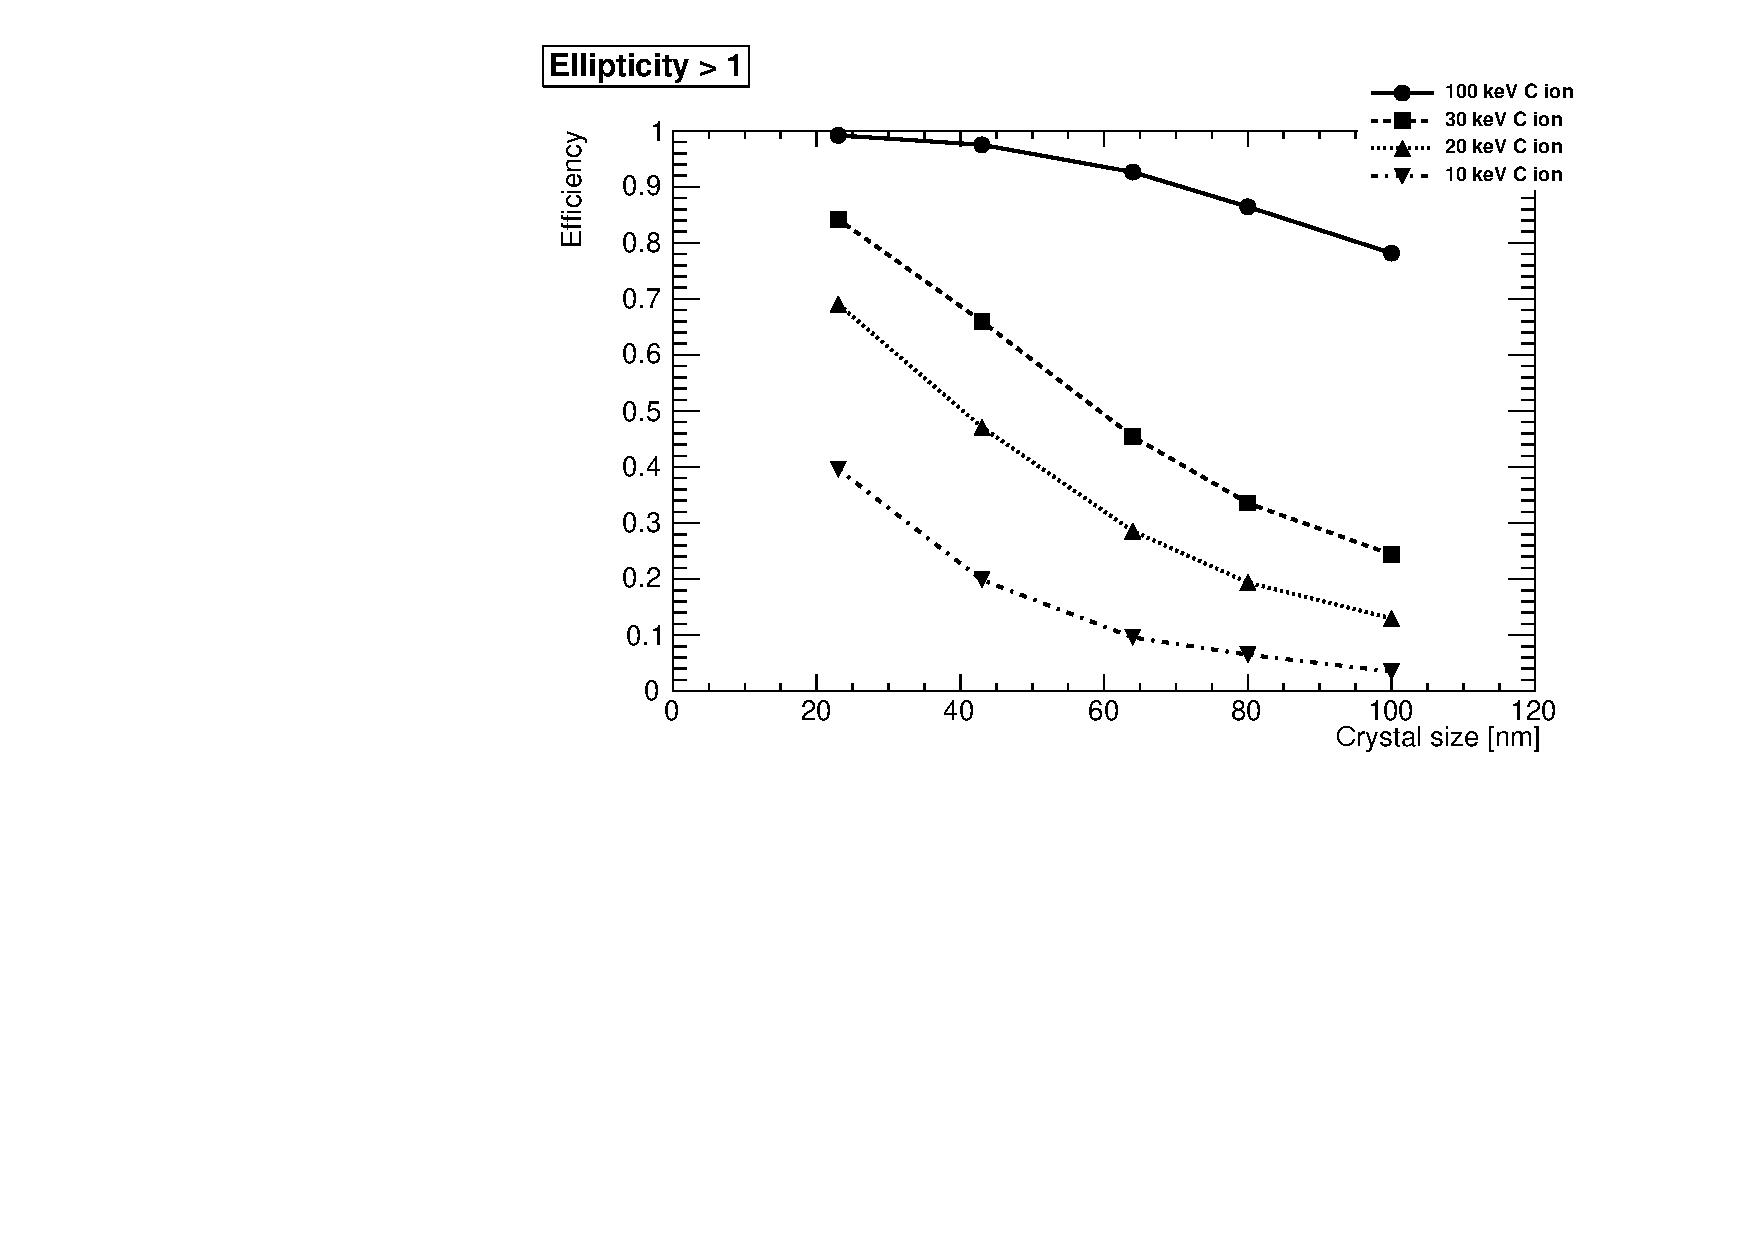
\includegraphics[angle=270,width=70mm]{./figs/result.pdf}
  \caption{テスト画像, width=70mm}\label{fig:test_image}
\end{figure}
\end{verbatim}
これを実際に描くと図~\ref{fig:test_image}のようになる。
\begin{figure}[htbp]
  \centering
  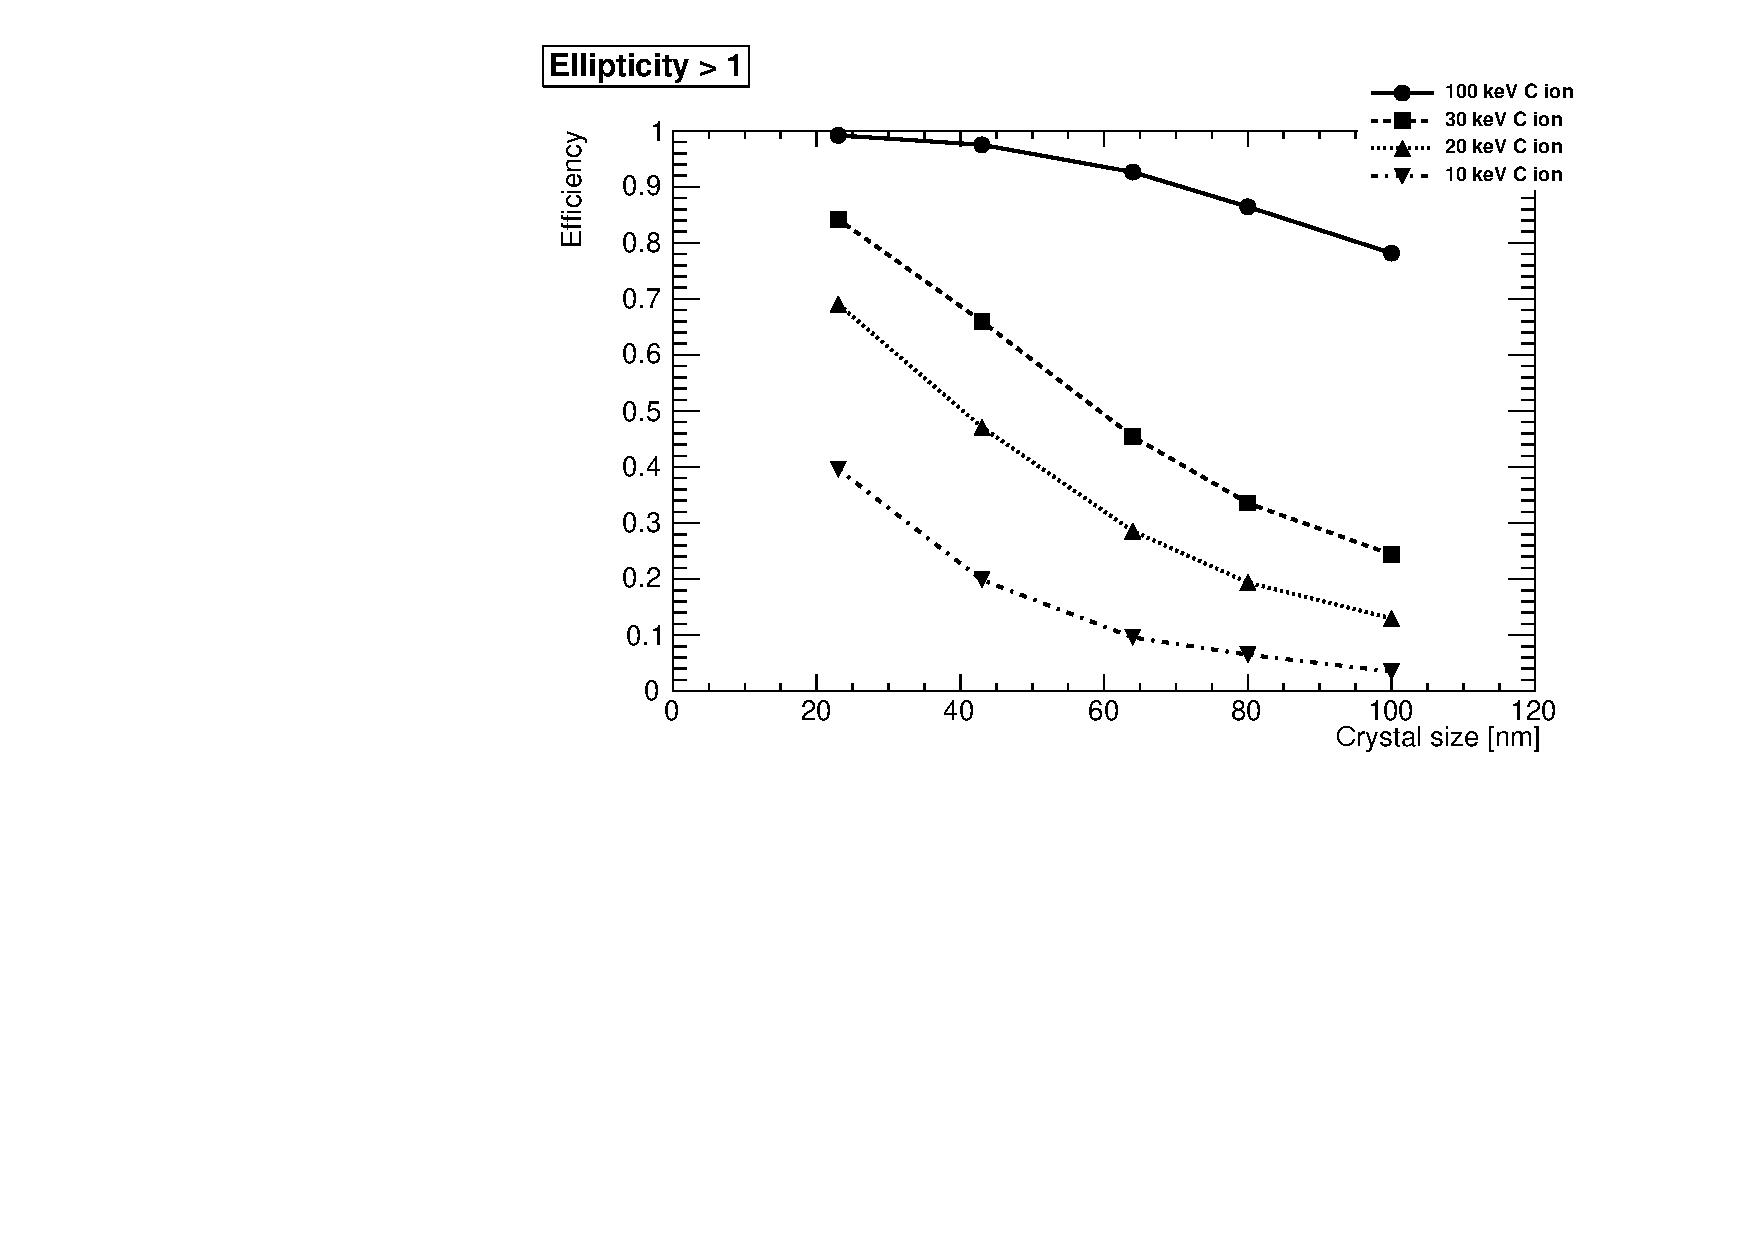
\includegraphics[angle=270,width=70mm]{./figs/result.pdf}
  \caption{テスト画像, width=70mm}\label{fig:test_image}
\end{figure}
画像のサイズの指定方法は、いくつかの方法がある。
\begin{verbatim}
width=100mm 幅をミリメートルで指定する方法
width=1.0\textwidth テキスト幅からの倍率で指定する方法
scale=0.2 画像やPDFファイルのサイズからの倍率を指定する方法
\end{verbatim}

当方の環境だとPDFは270度回転でいつも見ている角度になった。なのでPDFファイルの場合は\verb|angle=270|が必要かもしれない。


複数の画像を一つの図に表示させる方法がある。図~\ref{fig:various_angle_multi_images}で例を描画した。ソースはsample.texを参照されたし。

\begin{figure}[htbp]
 \begin{minipage}[b]{0.32\linewidth}
  \centering
  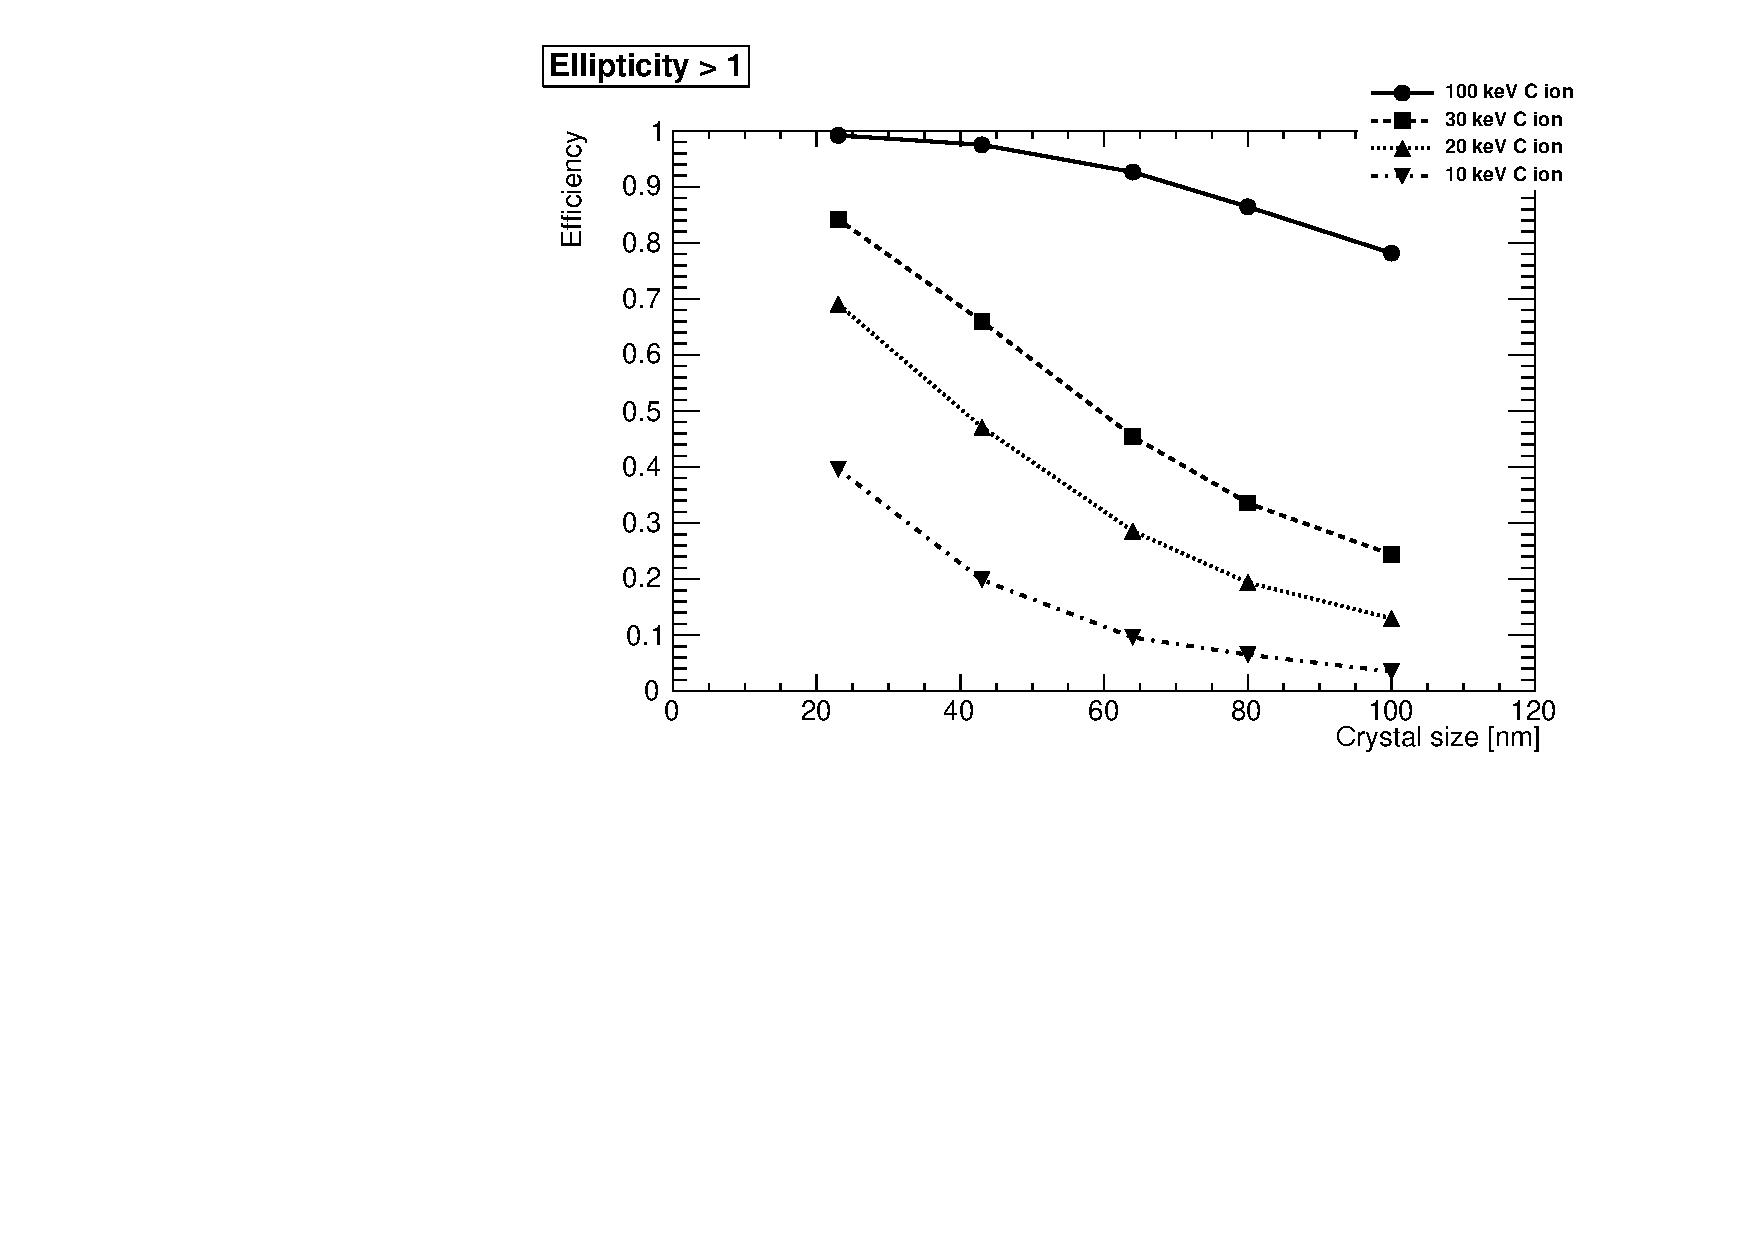
\includegraphics[angle=0,scale=0.2]{./figs/result.pdf}
  \subcaption{0deg}\label{0deg}
 \end{minipage}
 \begin{minipage}[b]{0.32\linewidth}
  \centering
  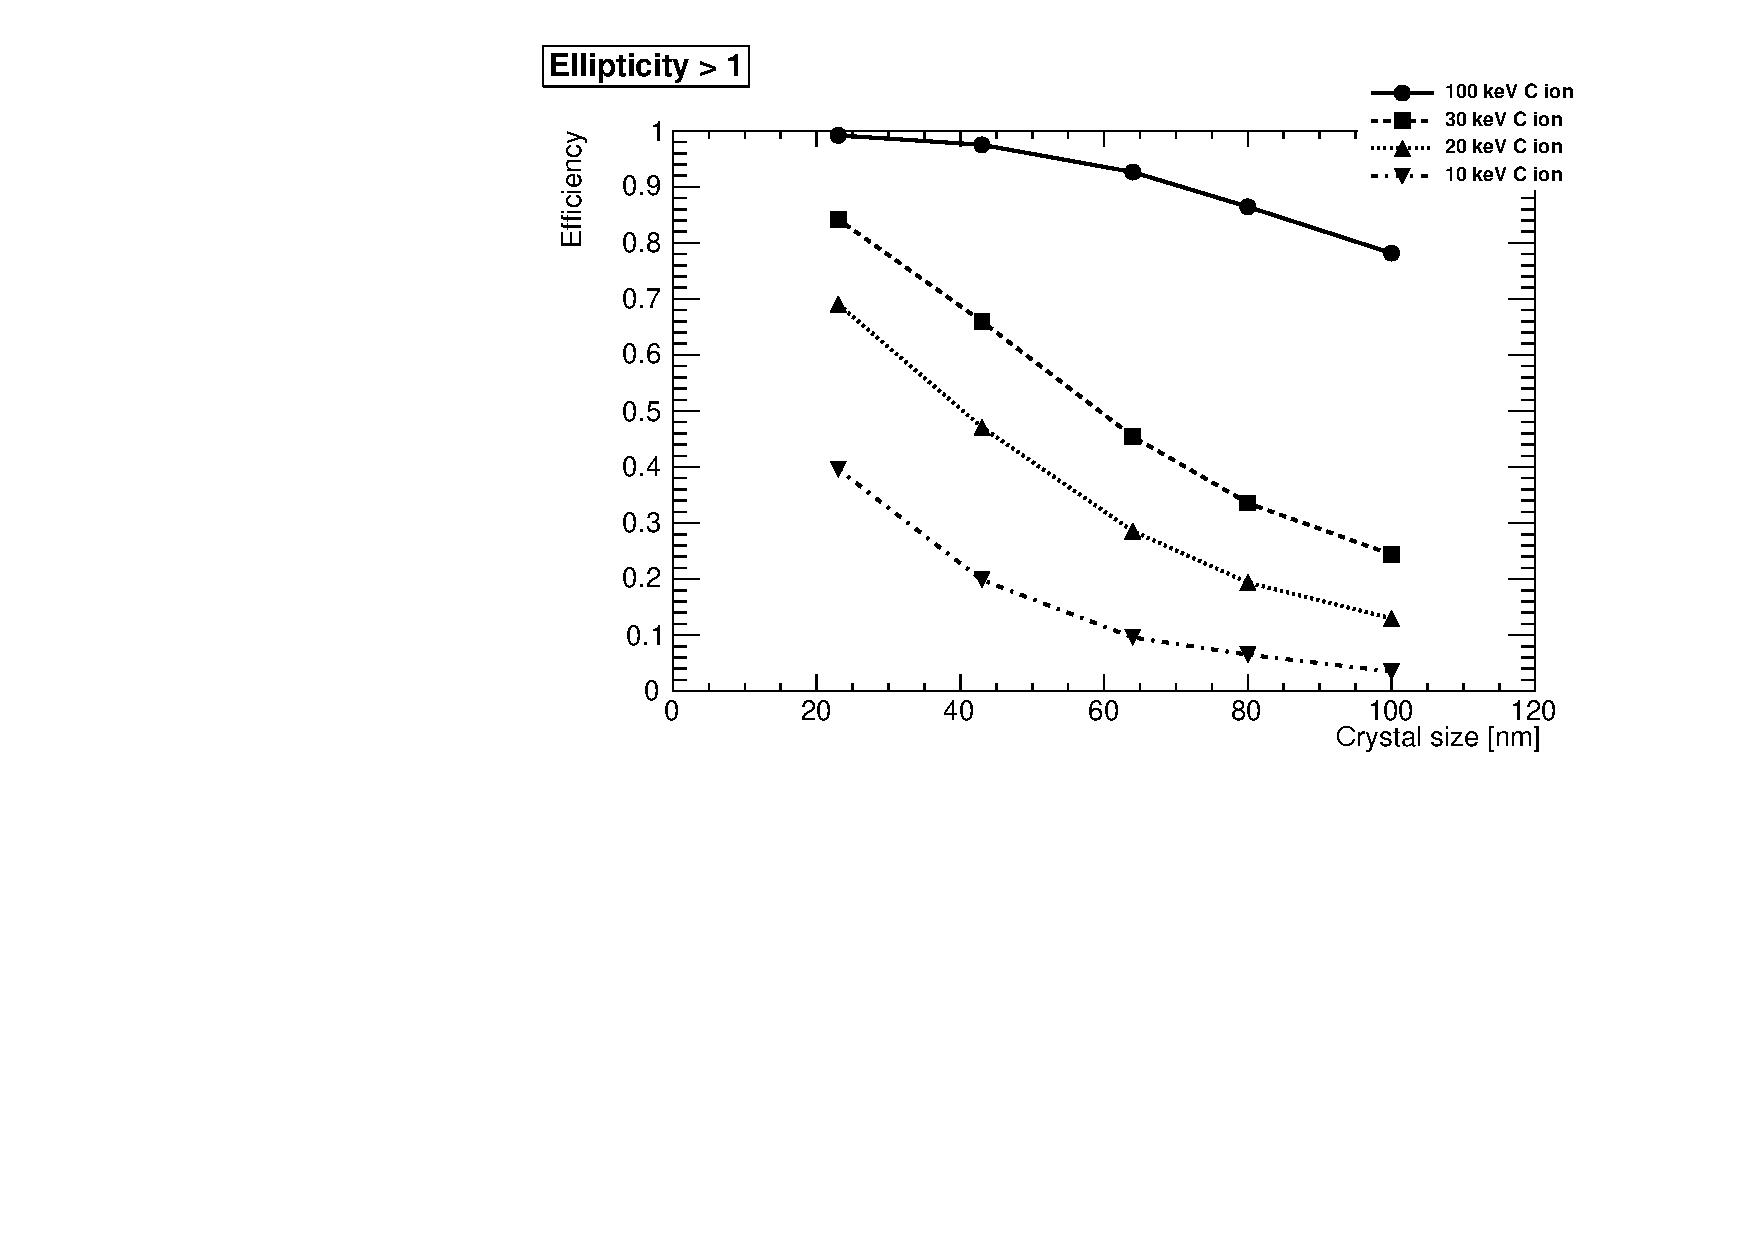
\includegraphics[angle=45,scale=0.2]{./figs/result.pdf}
  \subcaption{45deg}\label{45deg}
 \end{minipage}
 \begin{minipage}[b]{0.32\linewidth}
  \centering
  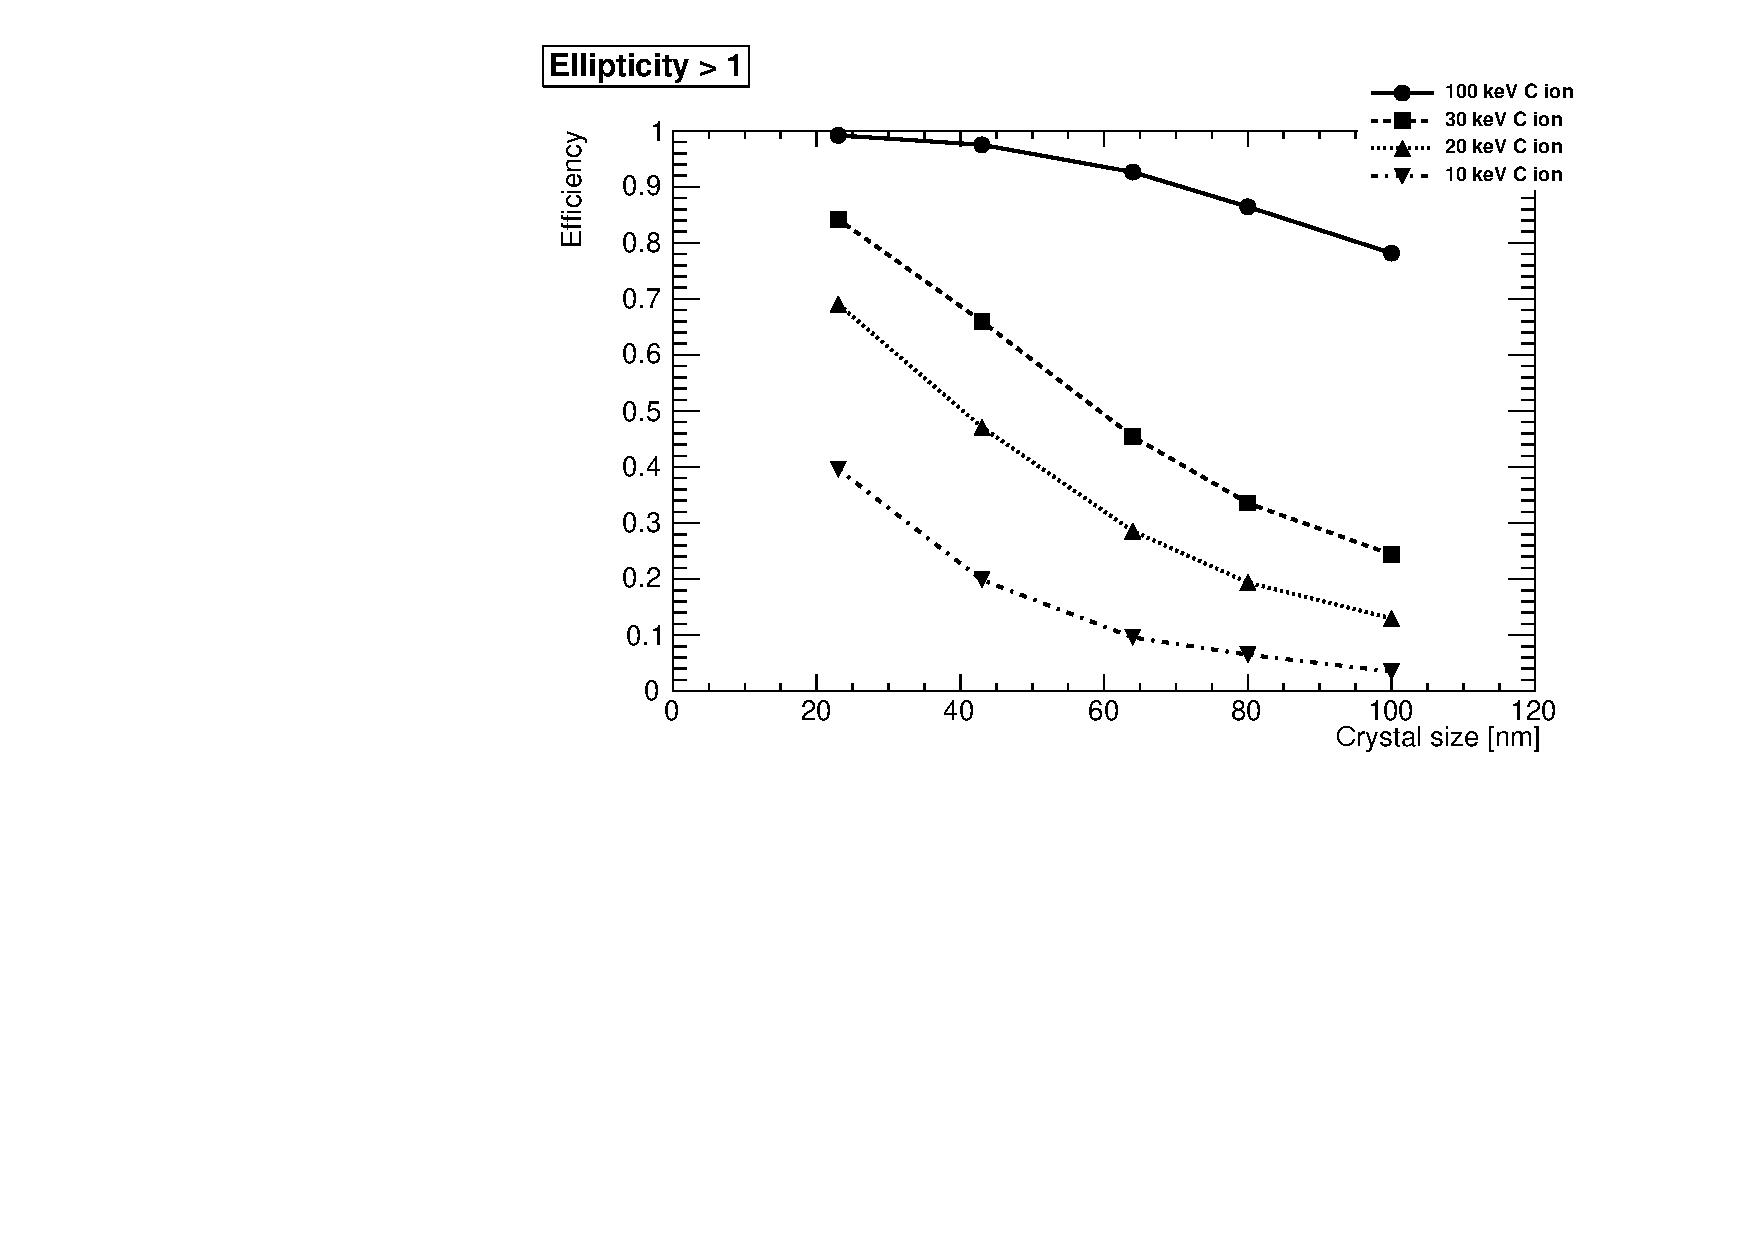
\includegraphics[angle=90,scale=0.2]{./figs/result.pdf}
  \subcaption{90deg}\label{90deg}
 \end{minipage}\\
 \begin{minipage}[b]{0.32\linewidth}
  \centering
  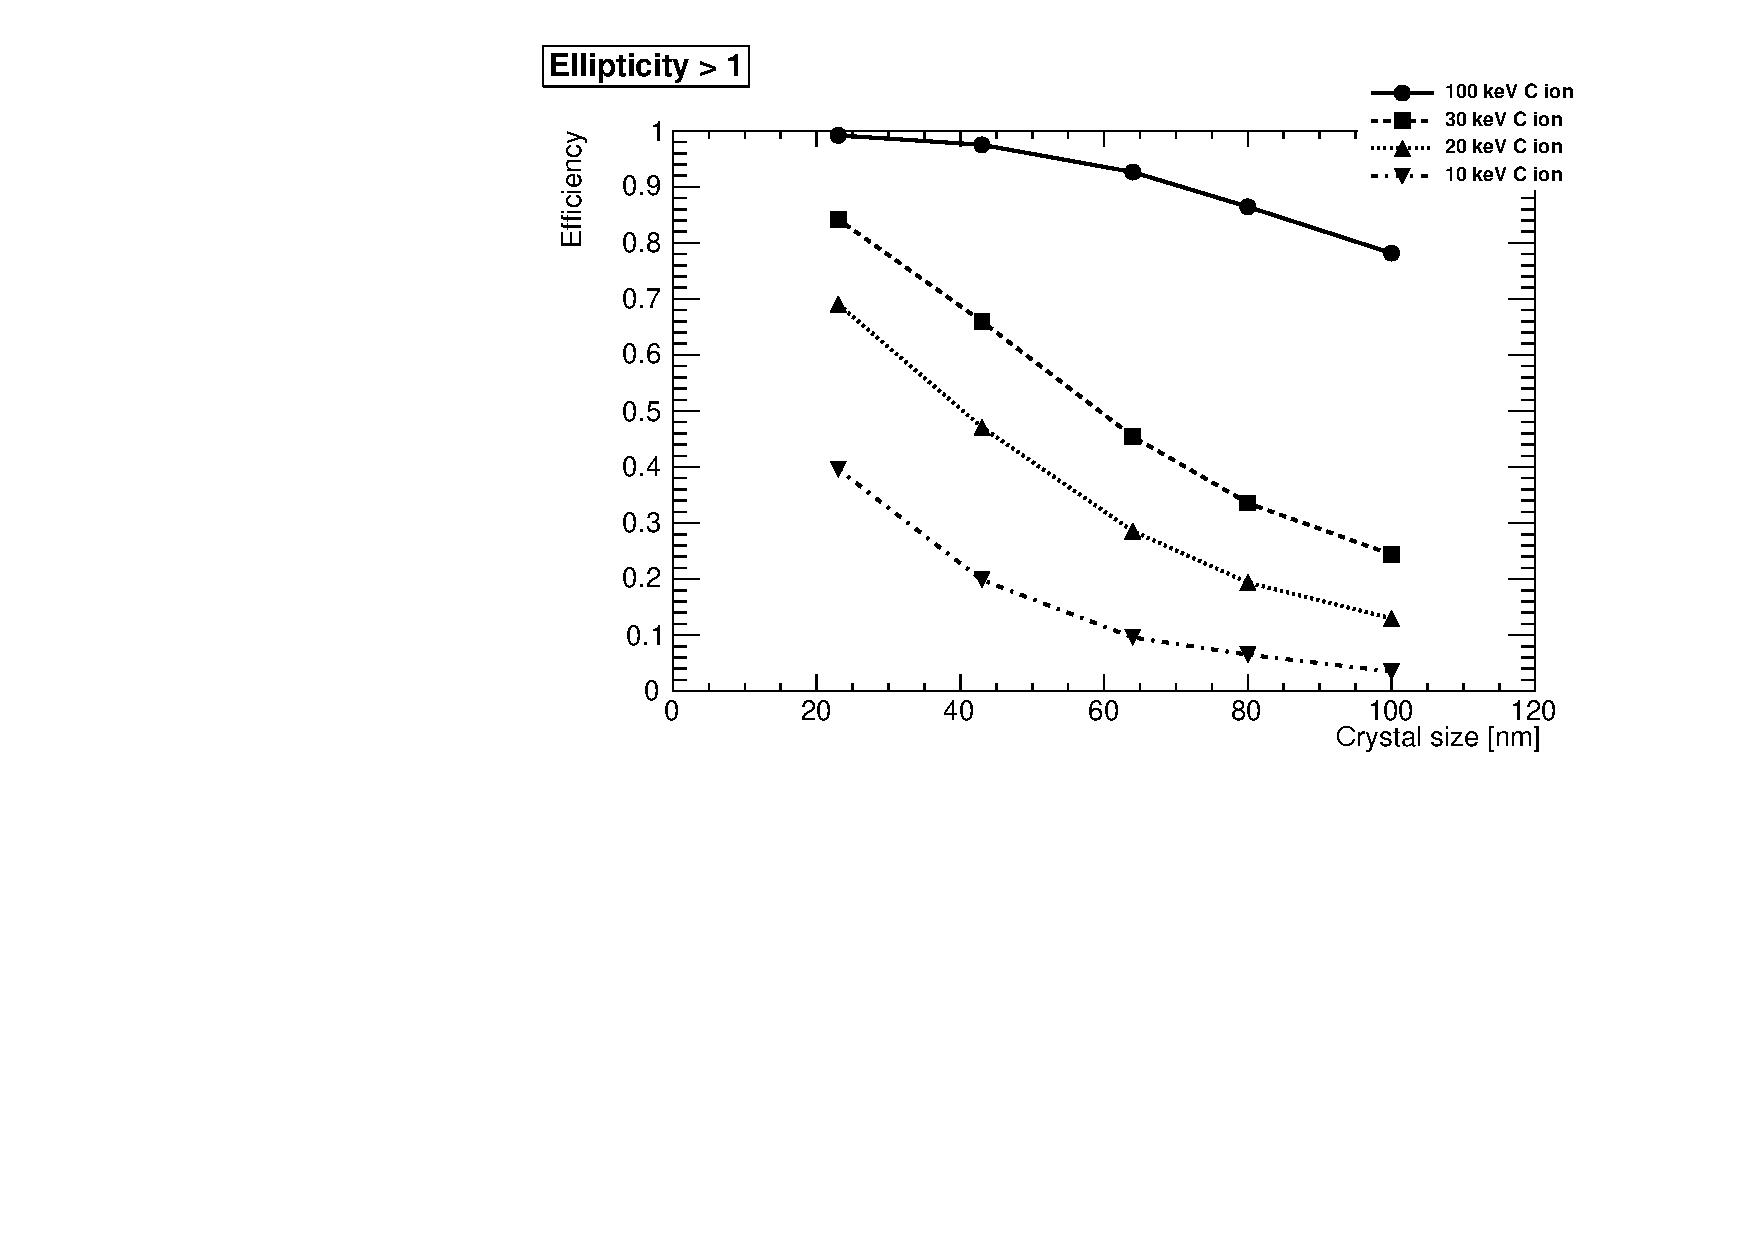
\includegraphics[angle=180,scale=0.2]{./figs/result.pdf}
  \subcaption{180deg}\label{180deg}
 \end{minipage}
 \begin{minipage}[b]{0.32\linewidth}
  \centering
  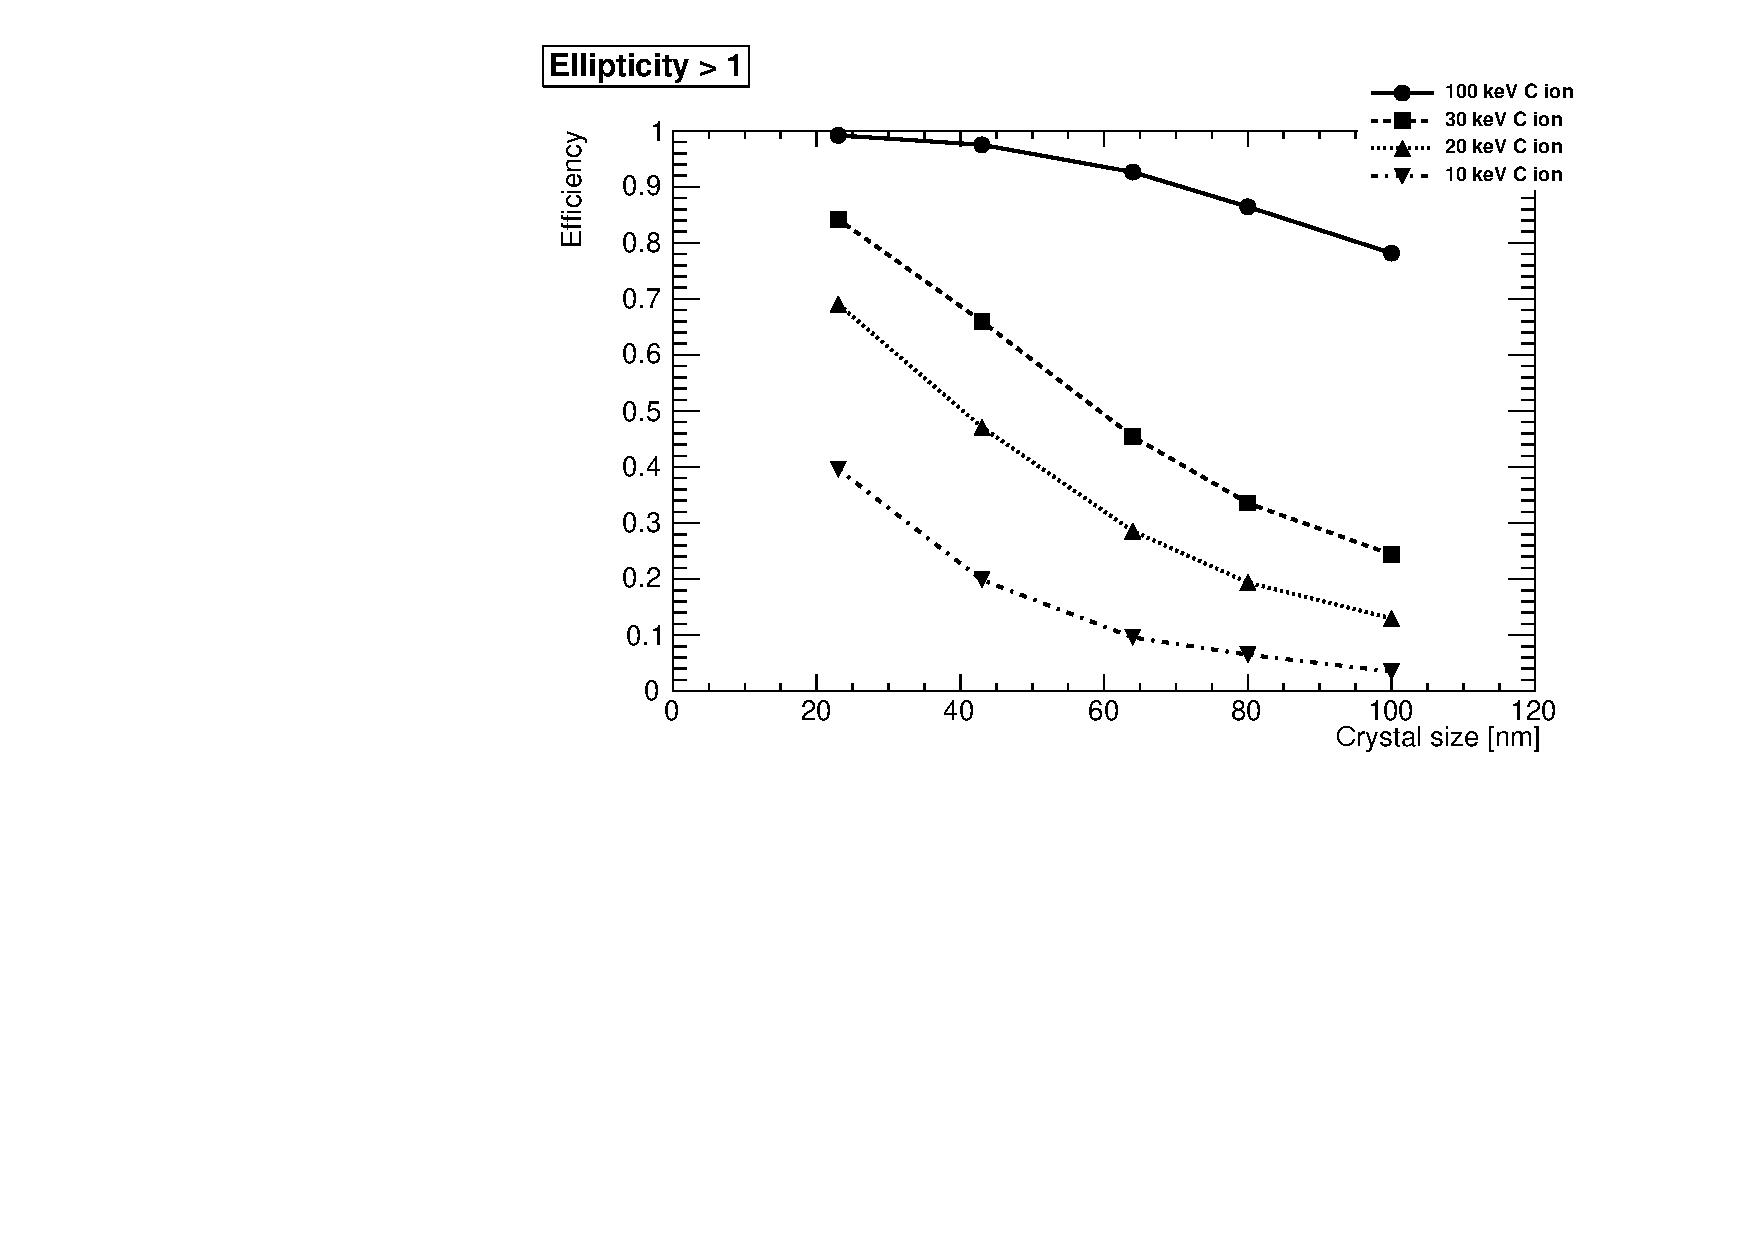
\includegraphics[angle=270,scale=0.2]{./figs/result.pdf}
  \subcaption{270deg}\label{270deg}
 \end{minipage}
 \caption{画像を回転させたり、複数の画像を表示する方法}\label{fig:various_angle_multi_images}
\end{figure}

グラフを作るときは、論文化しやすいようにPDFファイルで保存しておくと良い。他の形式ももちろん使える。図~\ref{fig:various_extension}で例を描画した。それぞれ異なる拡張子で表示してみた。

\begin{figure}[htbp]
 \begin{minipage}[b]{0.32\linewidth}
  \centering
  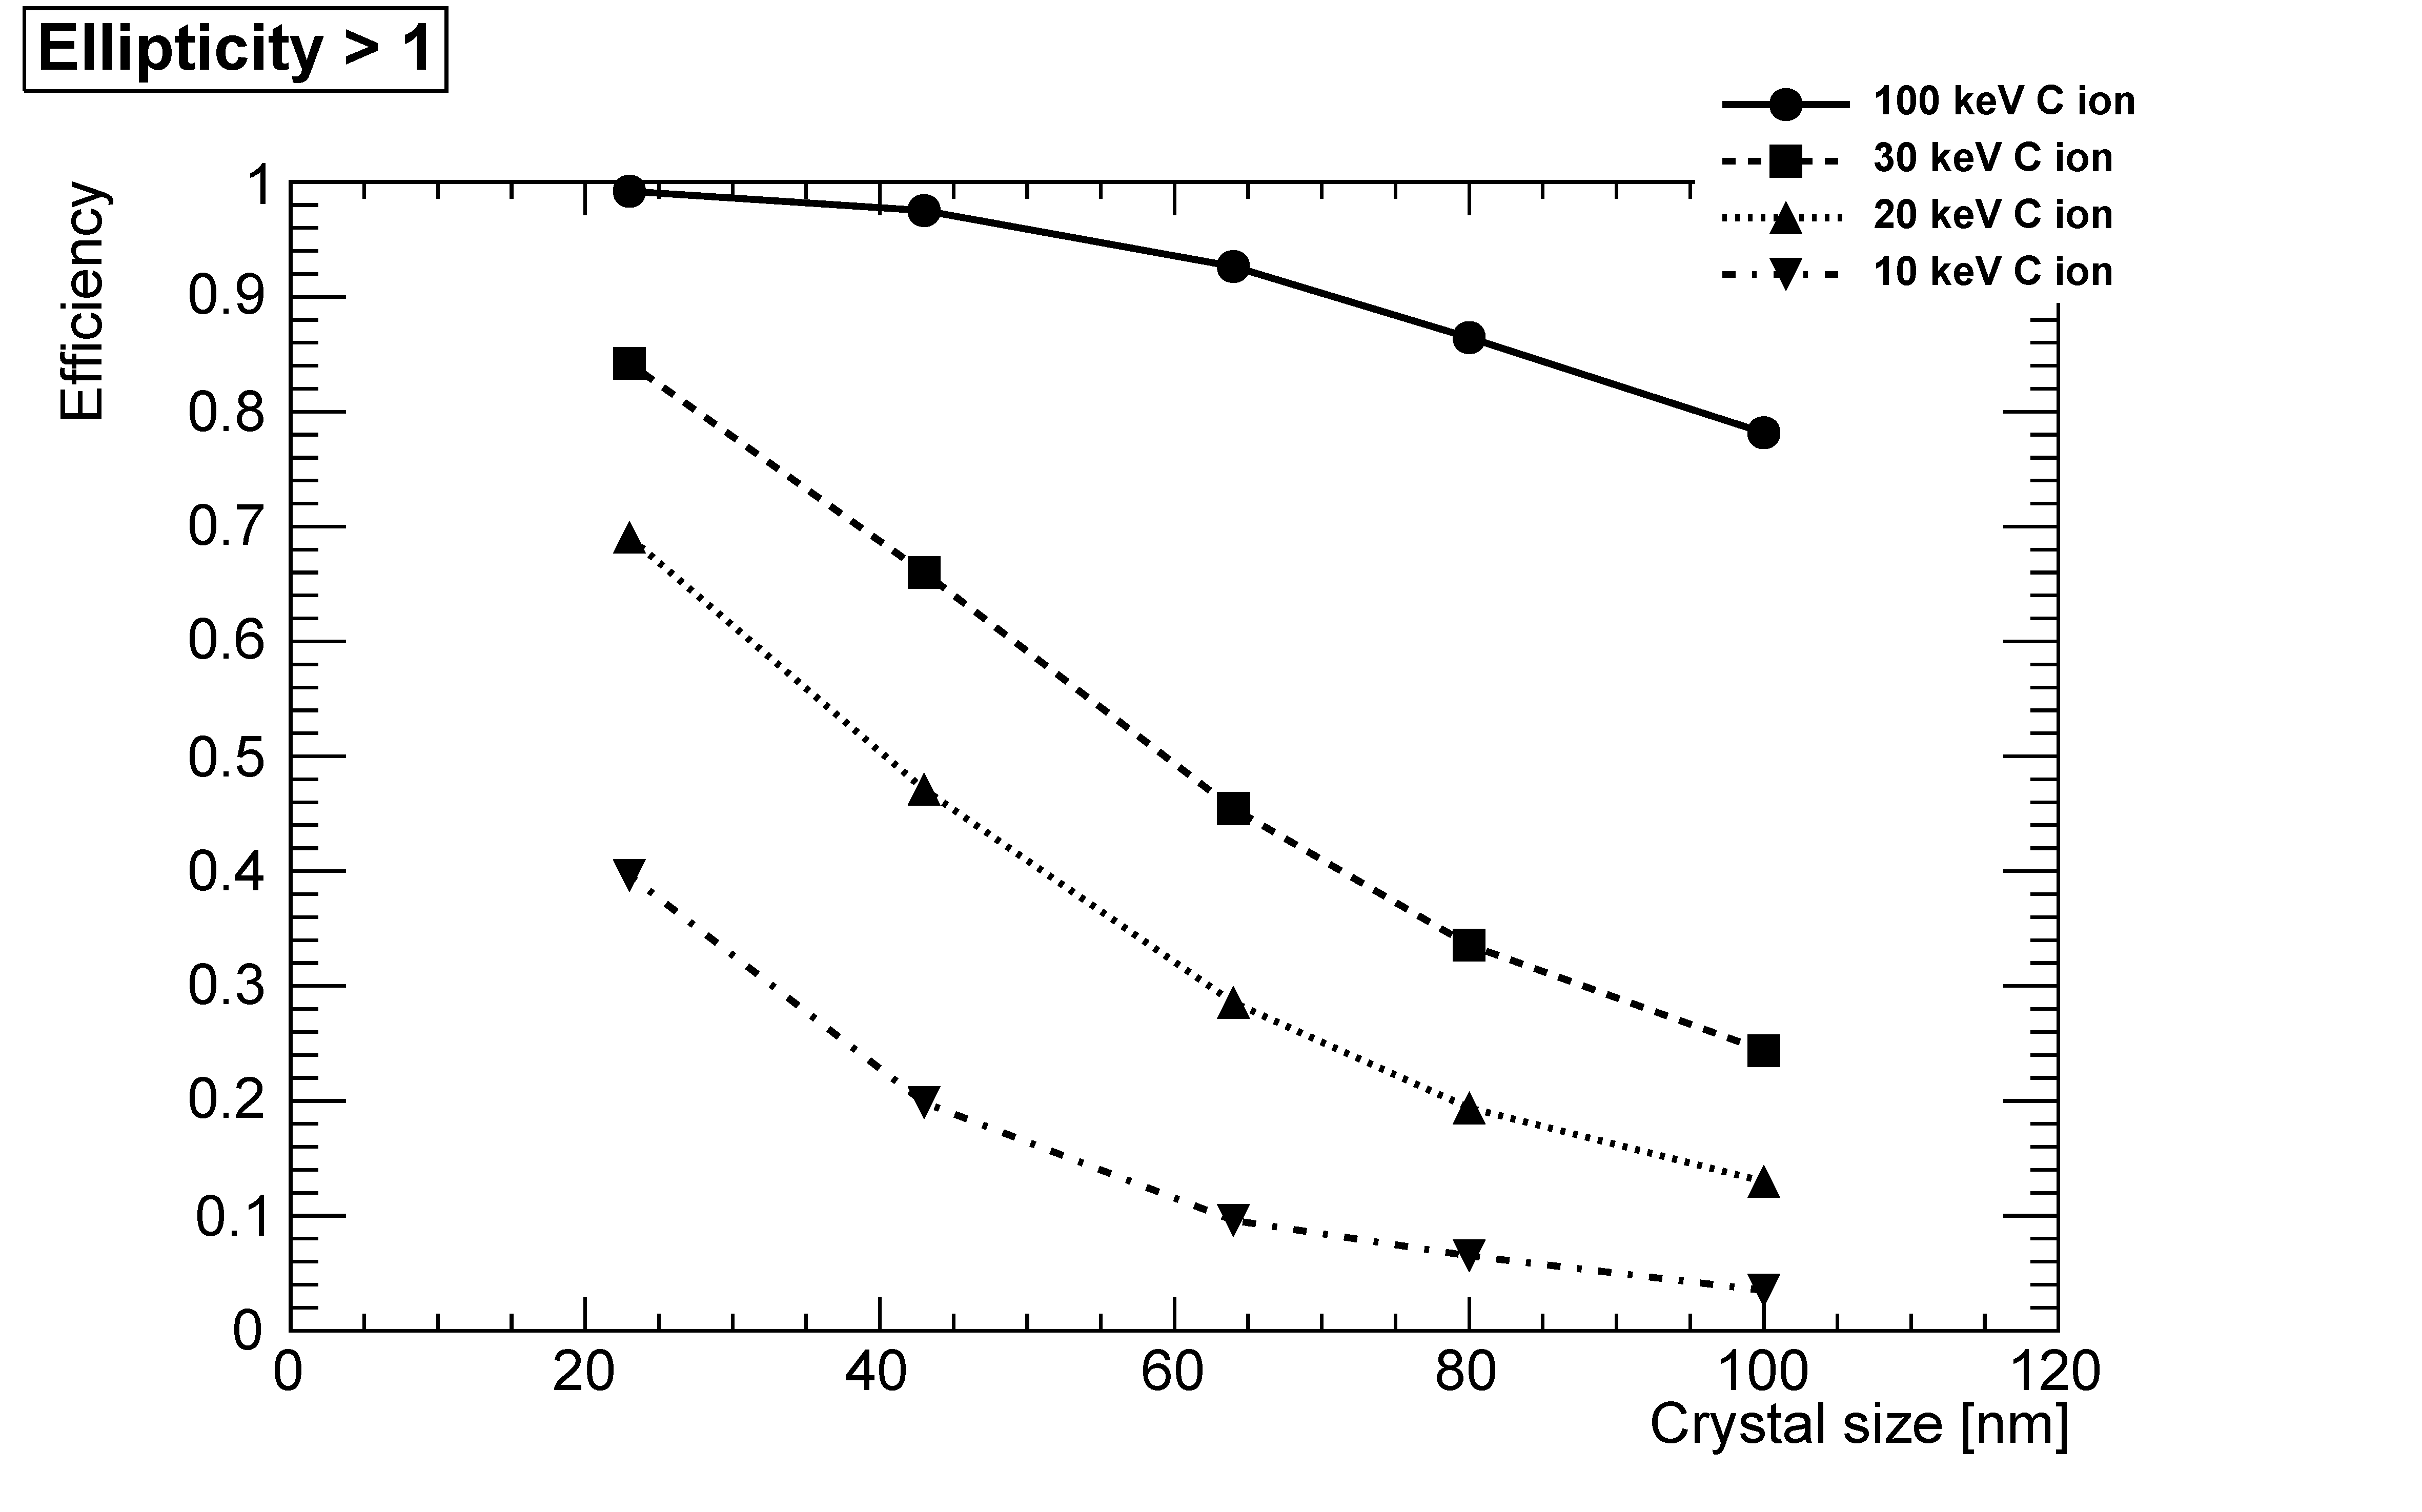
\includegraphics[angle=0,width=1.0\textwidth]{./figs/result.png}
  \subcaption{PNG}
 \end{minipage}
 \begin{minipage}[b]{0.32\linewidth}
  \centering
  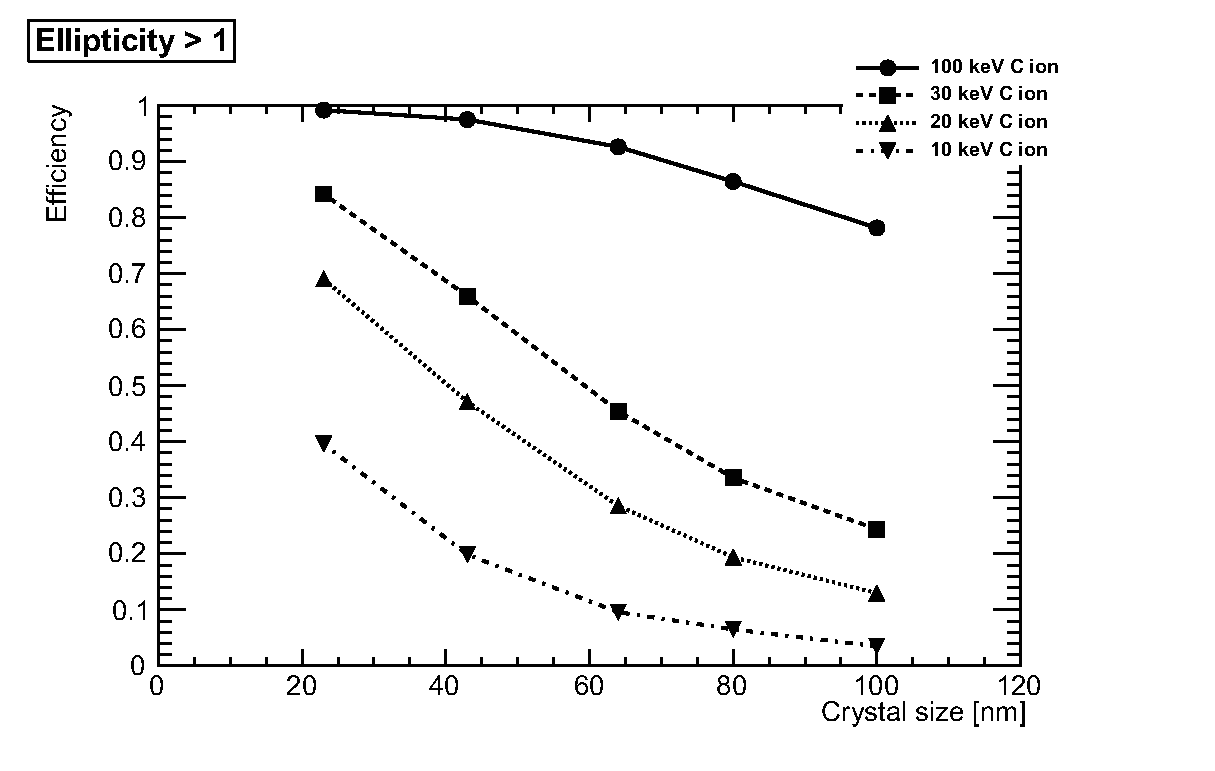
\includegraphics[angle=0,width=1.0\textwidth]{./figs/result.eps}
  \subcaption{EPS}
 \end{minipage}
 \begin{minipage}[b]{0.32\linewidth}
  \centering
  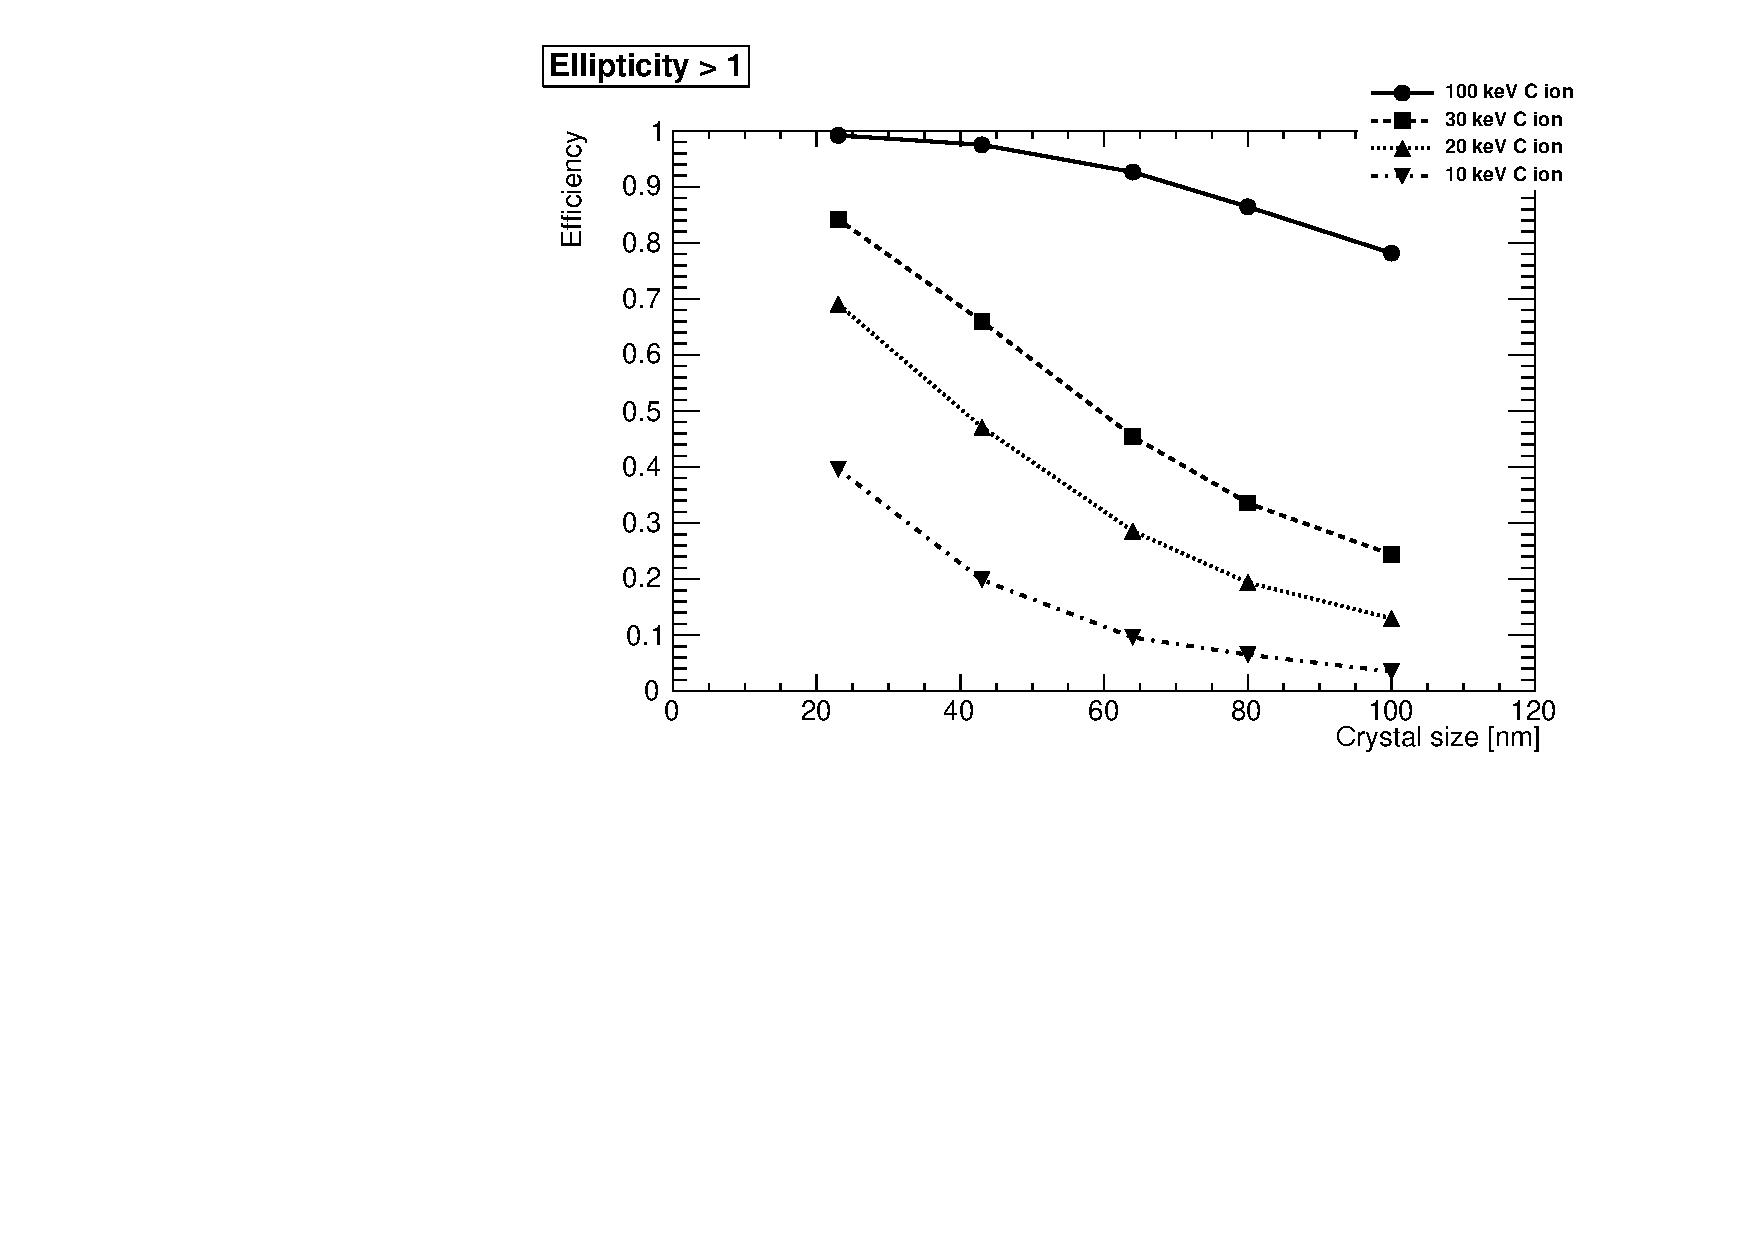
\includegraphics[angle=270,width=1.0\textwidth]{./figs/result.pdf}
  \subcaption{PDF}
 \end{minipage}\\
 \caption{png, eps, pdfで画像を表示する方法}\label{fig:various_extension}
\end{figure}

複数ページを持つPDFは、ページ番号を指定しながら表示させることが可能。図~\ref{fig:multi_page}で例を描画した。図~\ref{fig:page1}は1ページ目、図~\ref{fig:page2}は2ページ目。

\begin{figure}[htbp]
 \begin{minipage}[b]{0.5\linewidth}
  \centering
  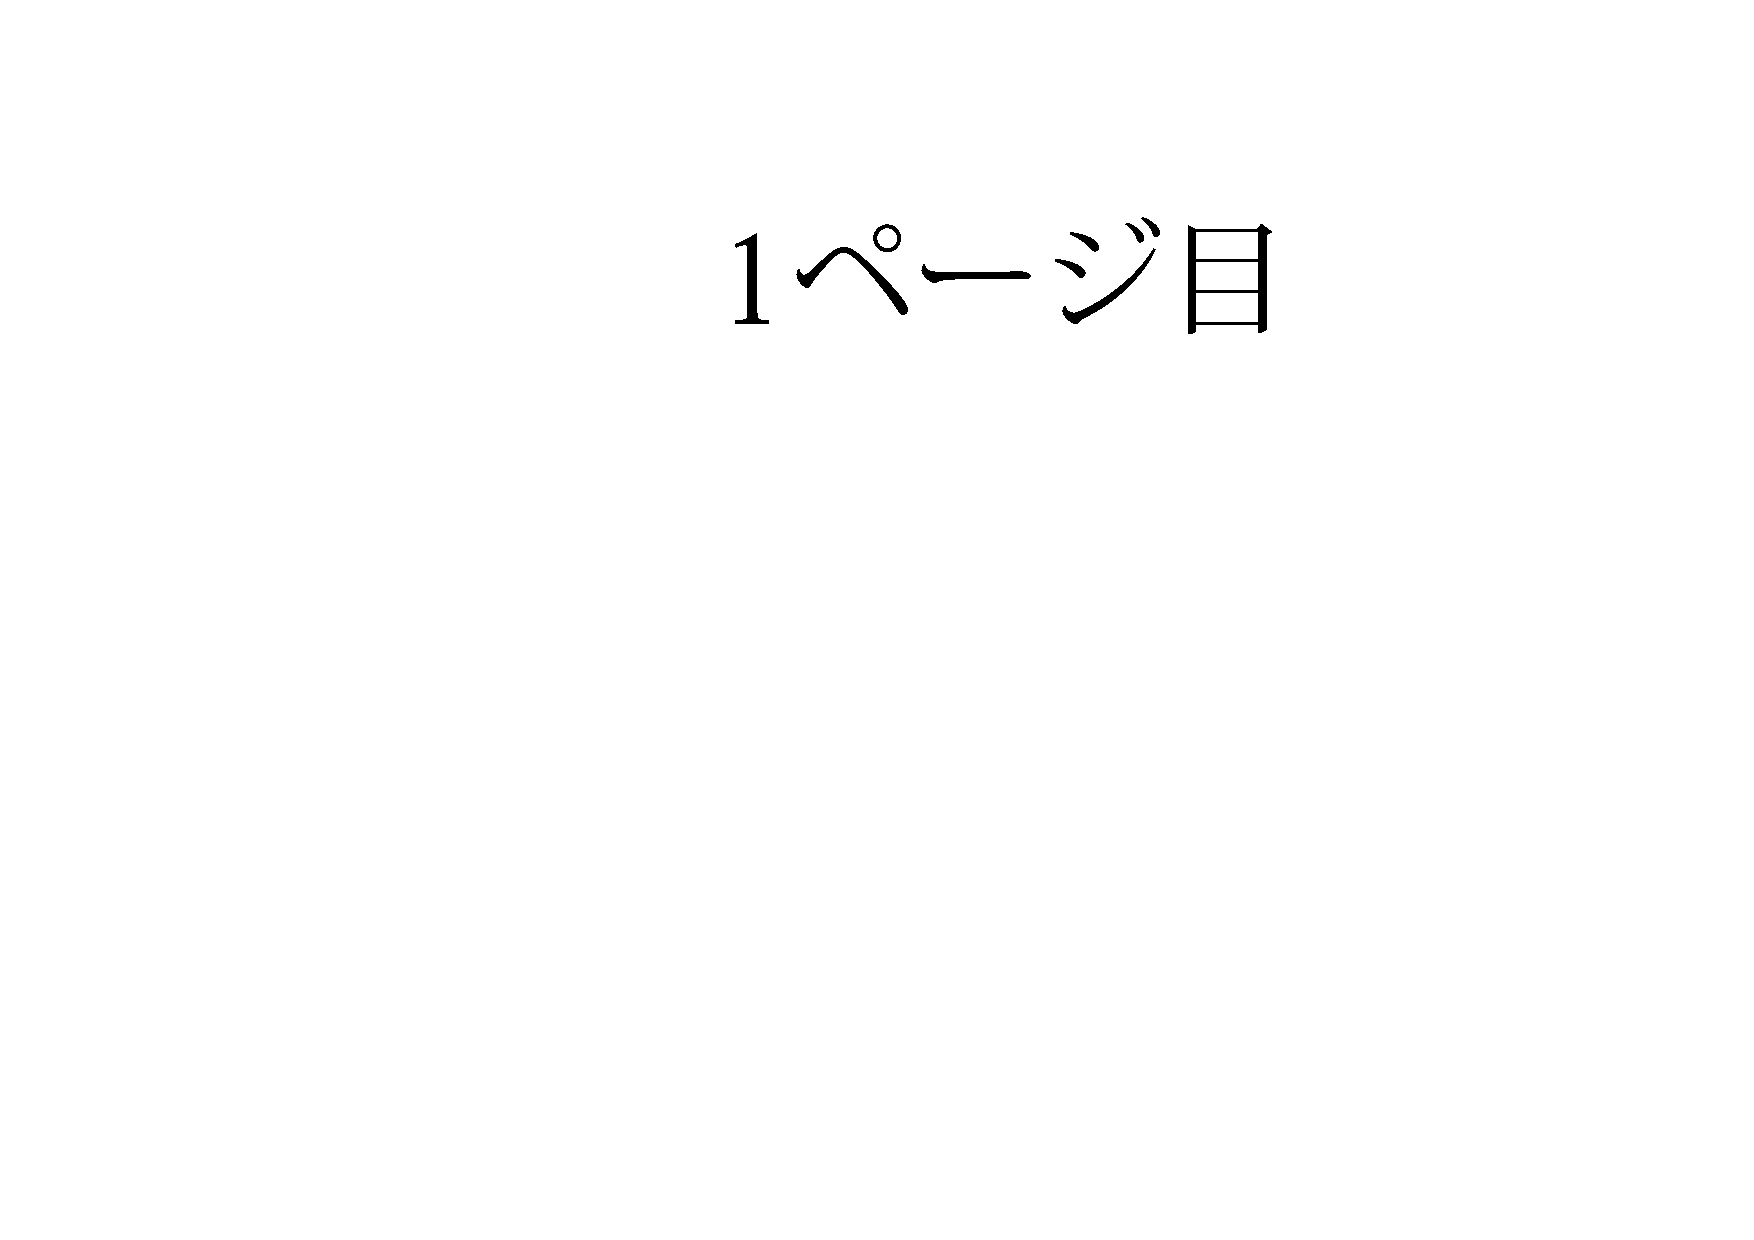
\includegraphics[angle=270,page=1,width=1.0\textwidth]{./figs/multi_page.pdf}
  \subcaption{multi\_page.pdfの1ページ目}\label{fig:page1}
 \end{minipage}
 \begin{minipage}[b]{0.32\linewidth}
  \centering
  \includegraphics[angle=270,page=2,width=1.0\textwidth]{./figs/multi_page.pdf}
  \subcaption{multi\_page.pdfの2ページ目}\label{fig:page2}
 \end{minipage}
 \caption{複数ページを持つPDFの一部を表示させる方法。}\label{fig:multi_page}
\end{figure}
\newpage
\section{テーブル}
テーブルは表~\ref{tab:emulsion_telescope}のように書く。詳細はググって。
\begin{table}[htbp]
\centering
	\begin{tabular}{r|c|l}
		右寄せ&中央寄せ&	左寄せ			\\
			&Fermi-LAT&	GRAINE			\\
		\hline
		\hline
		角度分解能@100~MeV	&105~mrad (6.0$^\circ$ ) &17~mrad (1.0$^\circ$ ) \\
		@1~GeV&16~mrad(0.90$^\circ$ )& 1.7~mrad(0.10$^\circ$) \\
		検出エネルギー範囲		&20--300~MeV		&10~MeV--100~GeV \\
		偏光感度		&無		&有 \\
		不感時間		&26.5~$\mu$sec (readout time) & 0\% \\
		\hline
	\end{tabular}
\caption{GRAINEエマルション望遠鏡の基本性能とFermi-LATとの比較}
\label{tab:emulsion_telescope}
\end{table}
\newpage
\section{リスト}
幾つかのリストを書く方法を示す。基本的にググれば全ての答えを得られる。itemize, enumerate, descriptionがよく使われる。
\subsection{itemizeを使う方法}
\begin{verbatim}
\begin{itemize}
 \item 調液
 \item 粒子形成
 \item 水洗+脱塩
\end{itemize}
\end{verbatim}

\begin{itemize}
 \item 調液
 \item 粒子形成
 \item 水洗+脱塩
\end{itemize}
\subsection{descriptionを使う方法}
\begin{verbatim}
\begin{description}
 \item [調液]\mbox{} \\調液とは、
 \item [粒子形成]\mbox{} \\粒子形成とは、
 \item [水洗+脱塩]\mbox{} \\水洗と脱塩とは、
\end{description}
\end{verbatim}
\begin{description}
 \item [調液]\mbox{} \\調液とは、
 \item [粒子形成]\mbox{} \\粒子形成とは、
 \item [水洗+脱塩]\mbox{} \\水洗と脱塩とは、
\end{description}
\subsection{enumerateを使う方法}
原子核乳剤の主な原料は・・・
\begin{verbatim}
\begin{enumerate}
 \item 硝酸銀 (高い)
 \item 臭化カリウム
\end{enumerate}
\end{verbatim}
\begin{enumerate}
 \item 硝酸銀 (高い)
 \item 臭化カリウム
\end{enumerate}
\newpage
\section{数式}
equation*で数式を書くとただの数式を書ける。
\begin{verbatim}
\begin{equation*}
a=b
\end{equation*}
\end{verbatim}
\begin{equation*}
a=b
\end{equation*}
equationで数式を書くと番号が付く。式~\ref{equ:ab}で例を示す。
\begin{verbatim}
\begin{equation}
a=b
\label{equ:ab}
\end{equation}
\end{verbatim}
\begin{equation}
a=b
\label{equ:ab}
\end{equation}
一粒子系のシュレーディンガー方程式を式~\ref{equ:oneparticle}で示す。
\begin{verbatim}
\begin{equation}
i\hbar\frac{\partial}{\partial t} \psi(\boldsymbol{x},t) = 
\left [ \frac{-\hbar^2}{2m}\nabla^2 + V(\boldsymbol{x},t)\right ] \psi(\boldsymbol{x},t)
\label{equ:oneparticle}
\end{equation}
\end{verbatim}
\begin{equation}
i\hbar\frac{\partial}{\partial t} \psi(\boldsymbol{x},t) = 
\left [ \frac{-\hbar^2}{2m}\nabla^2 + V(\boldsymbol{x},t)\right ] \psi(\boldsymbol{x},t)
\label{equ:oneparticle}
\end{equation}

\subsection{上付き下付き文字}
\begin{verbatim}
$x^a, x^{a+b}, x^{a^b}, a_i, a_{ij}, a_{i_j}$
\end{verbatim}
$x^a, x^{a+b}, x^{a^b}, a_i, a_{ij}, a_{i_j}$

\subsection{不等号}
\begin{verbatim}
$\sim, \simeq, >, <, \geq, \leq, \gg, \ll$
\end{verbatim}
$\sim, \simeq, >, <, \geq, \leq, \gg, \ll$

\subsection{演算子}
\begin{verbatim}
$+, -, \times, \div, \pm, \mp, \circ, \cdot$
\end{verbatim}
$+, -, \times, \div, \pm, \mp, \circ, \cdot$

\subsection{平方根}
\begin{verbatim}
$\sqrt{x}, \sqrt[n]{x}$
\end{verbatim}
$\sqrt{x}, \sqrt[n]{x}$

\subsection{ギリシャ文字}
\begin{verbatim}
$\Gamma, \Delta, \Theta, \Lambda, \Xi, \Pi, \Sigma, \Upsilon, \Phi, \Psi, \Omega$
\end{verbatim}
$\Gamma, \Delta, \Theta, \Lambda, \Xi, \Pi, \Sigma, \Upsilon, \Phi, \Psi, \Omega$

\begin{verbatim}
$\alpha, \beta, \gamma, \delta, \epsilon, \zeta, \eta, \theta, \iota, \kappa, \lambda, $\\
$\mu, \nu, $\xi, o, \pi, \rho, \sigma, \tau, \upsilon, \phi, \chi, \psi, \omega, $
\end{verbatim}
$\alpha, \beta, \gamma, \delta, \epsilon, \zeta, \eta, \theta, \iota, \kappa, \lambda, $\\
$\mu, \nu, \xi, o, \pi, \rho, \sigma, \tau, \upsilon, \phi, \chi, \psi, \omega, $
\subsection{行列}
\begin{verbatim}
\begin{equation}
 \begin{array}{rrr}
-1 & \ldots & 3 \\
\vdots & \ddots & 600 \\
  7 & 8 & -9
 \end{array}
\end{equation}
\end{verbatim}

\begin{equation}
\begin{array}{rrr}
-1 & \ldots & 3 \\
\vdots & \ddots & 600 \\
7 & 8 & -9
\end{array}
\end{equation}
\subsection{括弧}
\verb|\left \right|を使うと\verb|[ ], ( ), { }, | $|\;|$等で囲まれる数式を正しく囲むことができる。
\begin{verbatim}
\begin{equation}
 \left [ \frac{0}{1} \right ] + [\frac{0}{1}]
\end{equation}
\end{verbatim}
\begin{equation}\left [ \frac{0}{1} \right ] + [\frac{0}{1}]\end{equation}
\subsection{数式中の空白や改行}
数式モードでは全ての空白は無視されるので、明示的に空白コマンドを使う。改行して=でそろえたい場合は\verb|\begin{split}\end{split}|を使い、\verb|\\|で改行、\verb|&|でそろえる場所を指定する。
\begin{verbatim}
\begin{equation}
\begin{split}
a&=|\;| 大きめの空白\\
b&=|\:| 中くらいの空白\\
c&=|\,| 小さめの空白\\
d&=|| 空白なし\\
e&=|\!| 負の空白
\end{split}
\end{equation}
\end{verbatim}
\begin{equation}
\begin{split}
a&=|\;| 大きめの空白\\
b&=|\:| 中くらいの空白\\
c&=|\,| 小さめの空白\\
d&=|| 空白なし\\
e&=|\!| 負の空白
\end{split}
\end{equation}
\subsection{総和・総乗}
\begin{verbatim}
\begin{equation} f(x) = \sum_{i=0}^n x_i \end{equation}

\begin{equation}  f(x) = \prod_{i=0}^n x_i \end{equation}
\end{verbatim}
\begin{equation} f(x) = \sum_{i=0}^n x_i \end{equation}

\begin{equation}  f(x) = \prod_{i=0}^n x_i \end{equation}
\subsection{頻出表現}
\label{sec:frequent}
\noindent
角度 $^\circ$ = \verb|$^\circ$|\\
ミクロン $\mu m$ = \verb|$\mu m$|\\
数式中で斜体にしない $\rm{mm}$ = \verb|$\rm{mm}$|\\
ニュートリノ振動 $\nu_{\mu} \rightarrow \nu_{\tau}$ = \verb|$\nu_{\mu} \rightarrow \nu_{\tau}$|\\
臭化銀の沈殿 $\rm{KBr+AgNO_3\rightarrow AgBr\downarrow+KNO_3}$ = \verb|$\rm{KBr+AgNO_3\rightarrow AgBr\downarrow+KNO_3}$|
\subsection{Tips}
Wikipediaの数式は\LaTeX  の数式表記になっているので、欲しい関数は編集からソースを見るとよい。一粒子系のシュレーディンガー方程式もWikipediaからのパクりである。
\newpage
\section{その他}
\subsection{URL}
\verb|\begin{document}|の前に\verb|\usepackage{url}|が必要。
\begin{verbatim}
\url{http://flab.phys.nagoya-u.ac.jp}
\end{verbatim}
\url{http://flab.phys.nagoya-u.ac.jp}

\subsection{参照}
論文の参照は\verb|\cite{}|、図、テーブル、数式、セクションの参照は\verb|\ref{}|である。
\begin{verbatim}
アクライト~\cite{acrylite}、OPERAの論文~\cite{Agafonova:2014ptn}、頻出表現\ref{sec:frequent}
\end{verbatim}
アクライト~\cite{acrylite}、OPERAの論文~\cite{Agafonova:2014ptn}、頻出表現\ref{sec:frequent}

\subsection{他のページを読み込む}
別のファイルに中身を書いておいて、それをメインのファイルに統合することができる。inputはそのまま代入され、includeは読み込んだファイルの直前で改ページされる。使い方次第。拡張子\verb|.tex|は必要ない
\begin{verbatim}
\input{abst}
\include{abst}
\end{verbatim}

\subsection{一覧}
テーブルリスト\verb|\listoftables|、図のリスト\verb|\listoffigures|、参照はややこしいのでソースをみてほしい。
%\newpage %新しいページ
\listoftables %テーブルリスト
%\newpage %新しいページ
\listoffigures %図のリスト

\begin{thebibliography}{99}
\bibitem{acrylite}
\url{https://www.mrc.co.jp/acrylite/spec/index.html}
%\cite{Agafonova:2014ptn}
\bibitem{Agafonova:2014ptn}
  N.~Agafonova {\it et al.} [OPERA Collaboration],
  %``Observation of tau neutrino appearance in the CNGS beam with the OPERA experiment,''
  PTEP {\bf 2014} (2014) no.10,  101C01
  doi:10.1093/ptep/ptu132
  [arXiv:1407.3513 [hep-ex]].
  %%CITATION = doi:10.1093/ptep/ptu132;%%
  %44 citations counted in INSPIRE as of 23 Nov 2016
\end{thebibliography}

\end{document}
